\documentclass[upright, contnum]{umemoria}
\depto{CIENCIAS DE LA COMPUTACI\'ON}
\author{MAURICIO DANIEL QUEZADA VEAS}
\title{IDENTIFICACI\'ON DE CONTENIDO MULTIMEDIA RELEVANTE A PARTIR DE EVENTOS UTILIZANDO SU INFORMACI\'ON SOCIAL}
\auspicio{}
\date{ENERO 2013}
\guia{B\'ARBARA POBLETE LABRA}
\carrera{INGENIERO CIVIL EN COMPUTACI\'ON}
\comision{SERGIO OCHOA DELORENZI}{MAURICIO MAR\'IN CAIHUAN}{}

\usepackage{lipsum}
\usepackage{verbatim}

%\usepackage[latin1]{inputenc}
%\inputencoding{latin1}

%\usepackage[T1]{fontenc}
\usepackage{fontspec}
\usepackage{xunicode}
\usepackage{graphicx}

\usepackage[lined,boxed,commentsnumbered,ruled,vlined,portuguese,linesnumbered]{algorithm2e}
\usepackage{setspace}
\usepackage[all]{hypcap}
\usepackage{minted}
\usepackage{longtable}

% agrega bibliografia a la "Tabla de contenido"
\usepackage[nottoc,notlof]{tocbibind}

\usepackage{geometry}
\geometry{top=2cm, bottom=2cm, left=3cm, right=2cm}

\defaultfontfeatures{Mapping=tex-text}
%\setmainfont{Linux Libertine O}
\setmainfont{Linux Libertine O}
\setmonofont[Scale=1]{CMU Typewriter Text}

\renewcommand\listingscaption{Código}
\definecolor{bg}{rgb}{0.95,0.95,0.95}


\let\evensidemargin\oddsidemargin
\reversemarginpar

\begin{document}

\frontmatter
\maketitle

\begin{abstract}

Este trabajo consistió en el diseño e implementación de una metodología para la generación automática
de resúmenes de eventos a partir de documentos de contenido tanto textual como multimedial. La medida de relevancia para
la extracción de documentos representativos en el proceso de la generación de resúmenes consideró la inclusión de indicadores
\textit{sociales}, es decir, se consideran más importantes los documentos con mayor impacto en medios sociales, tal como
las redes sociales online.

El problema central fue la generación de resúmenes de eventos bien definidos, es decir, no se consideró el problema
de identificación de eventos en medios sociales. Para este trabajo, un evento se define como un acontecimiento que genera actividad en medios sociales. El resumen de un evento se construye principalmente a partir de una selección de documentos descriptivos que son publicados en los medios sociales en torno al evento en cuestión.

Se utilizó una estrategia de clustering particional para la identificación
de subtópicos de cada evento, y una estrategia simple para ponderar la relevancia de cada documento. Al no considerar
el contenido de los documentos, éstos pueden ser de tipo textual o multimedial, pudiendo generar resúmenes multimedia o visuales.
Este tipo de trabajo no ha sido profundamente estudiado en las áreas de investigación relacionadas a la fecha de esta memoria.

Se utilizaron los servicios de Google News y Last.fm para la obtención de eventos noticiosos y musicales, respectivamente.
Además, se utilizó la red social Twitter para el enriquecimiento y generación de documentos con información social. Se utilizó el
algoritmo de clustering K-means para la identificación de subtópicos mediante una representación adecuada de los documentos que
no considerara su contenido, de forma de generar un resumen visual de cada evento, y una estrategia simple para ordenar los resultados de acuerdo a relevancia de acuerdo a determinados indicadores sociales de los documentos.

La metodología fue evaluada sobre distintos eventos, tanto noticiosos como musicales, a partir de los cuales se generaron resúmenes multimediales automáticamente. También se analizaron casos puntuales manualmente, previa determinación de parámetros adecuados. Los resultados obtenidos indicaron que la calidad de los resultados no depende directamente de la cantidad de documentos utilizados, y que los indicadores sociales utilizados pueden ser calibrados para entregar más resultados relevantes. La metodología diseñada fue adecuada para alcanzar el objetivo principal, y puede ser mejorada en muchas aristas tanto en diseño como en implementación en el futuro.

\end{abstract}

\begin{dedicatoria}
Nunca supe qué poner aquí.
\end{dedicatoria}

\begin{thanks}
Quizás esta fue la parte más difícil de mi memoria. No porque el resto haya sido fácil, sino porque
intenté poner algo aquí novedoso, ingenioso, evitando los clichés y discursos de cada memoria, que son, dicho sea de paso, recitados de memoria:

\textit{Quisiera agradecer primero que nada a mi familia, a mis profesores que me han acompañado durante todo este trayecto; a mis amigos más cercanos... al estimado capitán del cuerpo de bomberos, autoridades políticas, eclesiásticas, civiles y militares... (léase con tono autoritario)}.

Realmente quienes me acompañaron de manera auténtica durante todo el comienzo de este viaje han sido dos cosas: el café y la falta de sueño. A ambos les agradezco darme el tiempo necesario para realizar este trabajo, y estoy seguro de que me seguirán acompañando en el futuro.

Al \emph{Smash}, a los \emph{miércoles de Gorbea}, a \emph{Los Talentosos Campesinos}, \emph{Jason Funk}, \emph{John Link}, \emph{Andy Briones}, al futuro \emph{dueño de una amasandería}, a \emph{Alce}, a \emph{Eulogio Villegas}, y a todos esos nombres que salen al escribir descuidadamente en un teclado o salidos de malas pronunciaciones o profecías apocalípticas.

Finalmente, no puedo evitarlo: a mis profesores, los que estuvieron y los que no; a los que ya no están (porque se fueron de viaje). A mis amigos, ellos saben quiénes son, y quiénes no (no, no es cierto, no saben). Y a mi familia, que sin su apoyo no habría podido llegar a escribir estas líneas, ni muchas otras que fueron y las que aún no han sido escritas.

\end{thanks}

\cleardoublepage
\begin{spacing}{1}

	\tableofcontents
	%\cleardoublepage
	%\listoftables
	%\cleardoublepage
	\listoffigures

\end{spacing}

% doble espaciado "makes a mess"
\setlength{\parskip}{\baselineskip}

\mainmatter


\chapter{Introducción}
\label{sec-1}


  Al igual que en el buffet de un restaurante, por mucho que se quisieran
  comer todos los platos, es imposible comer todo lo que uno
  quisiera por razones obvias. Una posibilidad es probar un poco de cada
  comida, para así saber qué es lo más delicioso y comer hasta
  hartarse.

  Pero, ¿qué hacer si hay demasiados platos y no se conocen todos? de
  alguna manera hay que saber cuáles hay que probar, si el objetivo es
  comer lo mejor posible. Para hacerse la idea de cuál 
  es la mejor oferta gastronómica del
  restaurant, sin tener que probar todos los platos, se puede
  preguntar a la gente que come habitualmente ahí qué platos fueron
  los que más les han gustado, y así definir la calidad de éste y/o
  escoger los mejores platos. Entonces se pueden escoger
  muestras de acuerdo a las recomendaciones.

  Pasando a un contexto diferente, supóngase que este gran buffet es la
  Web y los distintos platos corresponden a contenido publicado en
  ella. Por lo tanto, dada la gran cantidad de información disponible,
  se hace necesario poder encontrar lo más atractivo de acuerdo a la
  preferencia de los usuarios. Nótese que se está
  haciendo otra suposición importante con esta analogía, y es que se
  está considerando que la información es íntegramente para ser
  \emph{consumida}, y no, por ejemplo, para generar más contenido,
  conocimiento, para ser utilizada por máquinas, etc. Dentro de
  este contexto se plantea la pregunta de cómo seleccionar el contenido
  más atractivo dentro de todo lo que hay disponible en un momento dado. 
  O bien, filtrar los documentos que hablan de un mismo evento de acuerdo 
  a las preferencias de los usuarios, y luego presentarlo en la forma de 
  un \emph{resumen} de cada uno.

  Este trabajo consistió en el desarrollo de una metodología
  que permite generar resúmenes automáticos de eventos determinados
  a partir de los documentos Web que hablan de éstos. Un \emph{resumen} se
  considera como una selección de los documentos más representativos de un evento,
  lo cual permite describirlo con pocos elementos, en comparación a todos los que
  lo mencionan. A su vez, no se hace ninguna suposición sobre el \emph{contenido} de estos documentos (pueden
  ser de texto, imágenes, videos, \emph{multimedios} en general). Los
  documentos del resumen son seleccionados de acuerdo a
  \emph{indicadores sociales}: los elementos con mayor impacto en las redes
  sociales son considerados más importantes. 

  La metodología diseñada se implementó sobre dos tipos de eventos:
  noticias y conciertos musicales. Para obtenerlos, se utilizó
  el servicio de Google News\footnote{\href{http://news.google.com/}{http://news.google.com/} } y
  Last.fm\footnote{\href{http://last.fm/}{http://last.fm/} }. Los documentos y sus indicadores
  sociales se obtuvieron de la red social
  Twitter\footnote{\href{http://twitter.com/}{http://twitter.com/} }; y utilizando una representación
  adecuada de los documentos como vectores, se utilizó una estrategia
  de clustering para identificar los subtópicos de cada evento y así
  generar un resumen, basándose en los indicadores obtenidos. Esta memoria posee una 
  componente de investigación, al no estar del todo resuelto el problema 
  de la generación de resúmenes de contenido multimedia heterogéneo a partir de eventos.

  La estructura de este informe es como sigue: en este capítulo se
  comenta el contexto dentro del cual se desarrolló este sistema, las
  contribuciones realizadas, los objetivos y una descripción general
  de la solución. En Capítulo \ref{cap:antecedentes} se discute el estado del
  arte y el marco teórico del cual se desprende este trabajo. El
  Capítulo \ref{cap:problema} describe más en detalle el problema a resolver, su
  relevancia y sus dificultades. En el
  Capítulo \ref{cap:solucion} se describe la solución implementada, más
  un par de casos de estudio sobre los resultados obtenidos. Finalmente, las conclusiones 
  de este trabajo se encuentran en el Capítulo \ref{cap:conclusiones}.

\section{Contexto y Motivación}
\label{sec-1.1}


   La tasa de crecimiento de la cantidad de datos en la Web, y en
   particular, en las \emph{redes sociales online} (OSN, \emph{Online Social Networks}),
   es de tal magnitud que se vuelve necesario encontrar formas de
   filtrar y buscar sólo la información relevante dentro de todas las
   fuentes que hablan de un mismo acontecimiento. Por otra parte, 
   para poder entender lo que está pasando en el mundo a partir de los 
   puntos de vista de todas las personas o los hechos recabados en las redes
   sociales, se hace necesario poder procesar eficientemente estos 
   datos. Nuevamente, dado el gran volumen de datos, se vuelve 
   deseable el poder resumir esta información para ser rápidamente
   consumida.

   En el contexto de las redes sociales online, cada día los usuarios
   publican  millones de mensajes cortos con respecto a distintos
   tópicos, ya sean conversacionales, sobre eventos noticiosos,
   etc.\footnote{Pear Analytics. Twitter Study \href{http://es.scribd.com/doc/18548460/Pear-Analytics-Twitter-Study-August-2009}{http://es.scribd.com/doc/18548460/Pear-Analytics-Twitter-Study-August-2009} }
   Además, el auge de los teléfonos inteligentes o \emph{smartphones} con mayor
   capacidad de procesamiento e integrados con todo tipo de sensores
   (cámaras fotográficas, de vídeo, acelerómetro, osciloscopio, etc.),
   hace posible el generar aun más información y
   e incluso en tiempo real sobre lo que acontece en el mundo, en
   Internet, o bien sobre el estado particular de cada usuario.

   Este aumento y evolución de la generación de datos no sólo influye en la
   riqueza de éstos, sino también en el comportamiento de los usuarios
   a lo largo del tiempo. Actualmente,  una gran parte de éstos valora
   más el contenido de tipo multimedia (imágenes y videos)
   en las redes sociales online\footnote{The Rise of Visual Social Media \href{http://www.fastcompany.com/3000794/rise-visual-social-media}{http://www.fastcompany.com/3000794/rise-visual-social-media}. En el artículo se menciona un estudio sobre comportamiendo y preferencias de los usuarios en las redes sociales llevado a cabo por ROI Research: \href{http://www.slideshare.net/performics_us/performics-life-on-demand-2012-summary-deck}{http://www.slideshare.net/performics\_us/performics-life-on-demand-2012-summary-deck} }.
   Este contenido no sólo corresponde a documentos Web en el sentido
   tradicional, sino a objetos de más alto nivel como \emph{tweets}
   (mensajes cortos de la red social Twitter), imágenes (de servicios
   como Instagram\footnote{\href{http://instagr.am/}{http://instagr.am/} },
   Tumblr\footnote{\href{http://tumblr.com/}{http://tumblr.com/} }, etc.), vídeos
   (Youtube\footnote{\href{http://youtube.com/}{http://youtube.com/} }, Vimeo\footnote{\href{http://vimeo.com/}{http://vimeo.com/} }) e
   incluso sonidos (Soundcloud\footnote{\href{http://soundcloud.com/}{http://soundcloud.com/} }).
   Se hace entonces necesario encontrar formas para satisfacer estas
   necesidades de los usuarios, las cuales ya han sido
   abordadas en parte, como la generación de
   resúmenes automáticos orientado a motores de búsqueda, o la
   determinación de la relevancia tanto de documentos en la Web como de
   mensajes en las redes sociales.

   Surge como motivación el poder identificar y extraer contenido
   relevante de lo que está pasando en las redes sociales,
   clasificados dentro del concepto de eventos, y además avanzar un
   paso más arriba en el nivel de abstracción: considerar los
   documentos no por su contenido textual, lo que permite abarcar
   imágenes, vídeos, sonidos y multimedios en general. Algunas
   aplicaciones directas de esto son, entre otras:

\begin{itemize}
\item Ayudar al trabajo periodístico mediante una colección de
     contenido multimedia relacionado a un evento noticioso. Por
     ejemplo, la versión online de Radio
     Biobío\footnote{\href{http://www.biobiochile.cl/}{http://www.biobiochile.cl/} } frecuentemente publica
     breves artículos sobre sucesos que tienen impacto en las redes
     sociales, mostrando un pequeño conjunto de mensajes con
     comentarios de la gente\footnote{Como muestra: \href{http://www.biobiochile.cl/2012/12/01/aporte-de-lustrabotas-de-santiago-a-la-teleton-provoca-admiracion-en-redes-sociales.shtml}{http://www.biobiochile.cl/2012/12/01/aporte-de-lustrabotas-de-santiago-a-la-teleton-provoca-admiracion-en-redes-sociales.shtml}, y \href{http://www.biobiochile.cl/2012/12/01/rechazo-provocan-condicionamientos-de-compra-de-ripley-y-unimarc-para-donar-a-la-teleton.shtml}{http://www.biobiochile.cl/2012/12/01/rechazo-provocan-condicionamientos-de-compra-de-ripley-y-unimarc-para-donar-a-la-teleton.shtml} }.
     Una aplicación directa involucraría
     considerar además contenido multimedia, y organizar este
     contenido de acuerdo a la relevancia que tiene dentro de las
     redes.
\item Enriquecer la búsqueda en la Web a través de contenido
     multimedia. Una persona buscando información sobre un concierto
     podría obtener imágenes y vídeos de éste fácilmente una vez
     identificado el concierto.
\item Siguiendo lo anterior, un grupo musical podría obtener toda la
     información multimedia asociada a su concierto, tanto para sus
     fans como para ellos mismos, potenciando su popularidad.
\item Poder distinguir entre eventos similares rápidamente. Por
     ejemplo, un usuario que desee obtener información sobre ``Gaza'',
     puede referirse tanto a la banda de música como al conflicto en
     Israel. El poder distinguir rápidamente mediante una imagen o un
     vídeo acelera mucho el proceso. \emph{Una imagen vale más que mil palabras}.
\end{itemize}

  La metodología implementada está pensada como una primera aproximación para
  satisfacer los ejemplos mencionados.

\section{Objetivos}
\label{sec-1.2}

\subsection{Objetivo general}
\label{sec-1.2.1}


    El objetivo principal de este trabajo fue el siguiente:

    Diseñar e implementar un sistema que permita generar resúmenes
    automáticos de \emph{eventos}: información temporal publicada en redes
    sociales online sobre sucesos en particular. Esta información se
    basa en contenido textual y multimedial generado por los usuarios
    de estas redes, cuya relevancia esté basada en el impacto generado en
    éstas.


\subsection{Objetivos específicos}
\label{sec-1.2.2}


\begin{enumerate}
\item Extraer datos relacionados a eventos en la Web, principalmente
       aquellos generados en redes sociales online. Estos datos pueden
       componerse tanto de información textual como multimedial.
\item Agrupar la información extraída de un evento en subtópicos.
\item Seleccionar los elementos más relevantes de cada subtópico para
       producir un resumen del evento.
\item Analizar la efectividad de la metodología propuesta sobre un
       conjunto de eventos noticiosos y conciertos.
\end{enumerate}


\section{Descripción general de la solución}
\label{sec-1.3}


   Para enfrentar el problema se diseñó una solución que consiste en
   tres componentes, implementadas con diferentes
   grados de complejidad, siendo posible además mejorarlas en el
   futuro. Para probar la viabilidad de la metodología, ésta fue
   aplicada sobre un conjunto de casos de prueba.

   En particular:

\begin{itemize}
\item Se llevó a cabo un método para la obtención de documentos y
     enriquecerlos con datos obtenidos de fuentes sociales;
\item Se diseñó un procedimiento que separa estos documentos en
     \emph{clusters}, \emph{sin considerar su contenido}. Sólo se utilizó la
     información social asociada; y
\item Se diseñó además un procedimiento para \emph{rankear} u ordenar los
     resultados de acuerdo a \emph{relevancia}, siendo ésta medida de
     acuerdo a la información social asociada a los documentos
     generados.
\end{itemize}

% que quede el enumerate y su descriptor en la misma pagina
\newpage

   Las componentes diseñadas fueron las siguientes:

\begin{enumerate}
\item La que obtiene descripciones de eventos a partir de fuentes de
      éstos en la Web, enriqueciéndolos con información social;
\item Otra componente que procesa y separa los documentos a partir de
      la información social; genera \emph{objetos Web} y los separa en
      subtópicos de cada evento, respectivamente; y
\item La componente que entrega los $k$ documentos más relevantes por
      cada evento obtenido, basándose en los subtópicos identificados.
\end{enumerate}
\chapter{Antecedentes}
\label{sec-2}

\section{Twitter}
\label{sec-2.1}

Twitter es una red social online que permite conectar a
personas mediante la comunicación de mensajes cortos, rápidos y frecuentes. Estos
mensajes son publicados en el perfil del usuario que los emite, pueden
ser vistos directamente por los seguidores de este usuario o ser
vistos directamente en el perfil o buscándolos mediante una
funcionalidad que provee el servicio. Además, un usuario puede
\emph{seguir} a otros para poder ver en su \emph{timeline} los mensajes de todos
a quienes sigue.

FIGURA TWITTER

Estos mensajes, o \emph{tweets}, pueden además \emph{mencionar} a otros
usuarios, mediante la convención ``=@usuario [texto]='' indica que
se está mencionando a la persona con el nombre ``usuario''. Adicionalmente,
existen varias convenciones o costumbres que han surgido a lo largo
del tiempo en esta red desde sus inicios el año 2007:


\begin{itemize}
\item Respuestas o \emph{replies}: son mensajes del tipo \texttt{@usuario [texto]},
  que ocurren usualmente en una conversación entre dos usuarios.
\item Menciones o \emph{mentions}: un poco más general a una respuesta, el
  nombre del usuario mencionado puede estar en cualquier parte del
  mensaje. La diferencia semántica es que no se le habla
  ``directamente'' al usuario mencionado, como en una respuesta, sino
  que sólo es mencionado por si el mensaje es de su interés o no.
\item \emph{Retweets}: son mensajes del tipo \texttt{RT @usuario: [texto]}. Ocurren
  cuando se quiere compartir el mensaje de otro usuario, o citarlo
  para mencionarlo en el mismo mensaje.
\item \emph{Hashtags}: son palabras precedidas por el caracter \#, que indican
  un identificador a cierto evento o suceso dentro o fuera de la
  red. Suelen usarse para categorizar de cierta forma un tópico, pero
  son libres de usarse como los usuarios quieran.
\item Mensaje simple: un mensaje sin menciones ni hashtags.
\end{itemize}
Ejemplos:

\begin{itemize}
\item Mensaje simple: \texttt{Jason Funk disipa patitos};
\item Respuesta: \texttt{@jason estoy de acuerdo con lo que dices};
\item Mención: \texttt{creo que @jason es una cumbre de sabiduría};
\item Retweet: \texttt{RT @jason: Jason Funk disipa patitos}; y
\item Hashtag: \texttt{Estoy escribiendo mi memoria \#dcc \#summarization}
\end{itemize}
Estos mensajes están limitados a 140 caracteres de extensión. Sumando
esto a la integración de la red con otros servicios y dispositivos, y
a la cantidad de mensajes publicados cada minuto, permite utilizar
esta red como una gran fuente de datos.

Twitter además provee varios servicios adicionales, como por ejemplo,
un servicio de acortamiento de URLs, para permitir incluir una URL
larga sin perjudicar la cantidad de caracteres restantes para el
mensaje; un servicio de alojamiento de fotos y vídeos, para hacer más
sencilla la publicación de mensajes multimedia desde dispositivos
móviles; un servicio de búsqueda que permite buscar una cantidad
determinada de tweets sobre un término de búsqueda o un hashtag.


\section{Identificación automática de eventos}
\label{sec-2.2}

\section{Clustering de documentos}
\label{sec-2.3}

\subsection{Evaluación de clusterings}
\label{sec-2.3.1}

\section{Resúmenes automáticos}
\label{sec-2.4}

\subsection{Evaluación de resúmenes}
\label{sec-2.4.1}

\section{Ranking de documentos}
\label{sec-2.5}


\chapter{Especificación del Problema}
\label{sec-3}

\label{cap:problema}

  El problema a resolver consiste en poder \emph{resumir} eventos en base
  al contenido textual y multimedial de la información publicada en
  medios sociales, tales como las redes sociales online.

  Se considerará un evento como una ocurrencia en el mundo real
  con un período de tiempo asociado y un conjunto de mensajes, de
  volumen considerable, que discutan la ocurrencia y además publicados
  dentro del período de tiempo.

  El resumir un evento consiste en entregar un subconjunto de
  mensajes o de documentos mencionados en ellos que tengan
  relación directa con el evento en cuestión. Por ejemplo, el evento
  \texttt{Anef anuncia movilización nacional} contiene muchos mensajes, tales
  como:
\begin{itemize}
\item \texttt{RT @econtingencia: Reajuste: Trabajadores del sector público}
    \texttt{convocan a movilizaciones: La negociación entra a su recta final:}
    \texttt{El l... h ...}
\item \texttt{CUT de La Araucanía se adherirá a marcha nacional en rechazo a}
    \texttt{reajuste salarial: La Central Unitaria de}
    \texttt{Trabaja... http://t.co/IcgohlTR}
\item \texttt{Reajuste: Trabajadores del sector público convocan a}\\
    \texttt{movilizaciones http://t.co/pWC7q6NI}
\item \texttt{RT @biobio: CUT de La Araucanía se adherirá a marcha nacional en}
    \texttt{rechazo a reajuste salarial ofrecido por el Gobierno}
    \texttt{http://t.co/IOieDido}
\item \texttt{http://t.co/ttFp0XgH Trabajadores del sector público anuncian}
    \texttt{movilizaciones}
\item \texttt{RT @DanielaLopezLv: http://t.co/ttFp0XgH Trabajadores del sector}
    \texttt{público anuncian movilizaciones}
\item \texttt{RT @Barbara\_figue: Reajuste: Trabajadores del sector público}
    \texttt{convocan a movilizaciones http://t.co/DeXKACSR vía @nacioncl}
\end{itemize}
  El resumen consistirá en una colección de objetos, documentos o
  mensajes, donde en este caso los documentos están representados por
  las URLs contenidas en los mensajes, de forma que esta colección
  represente lo mejor posible el evento, siendo de tamaño
  considerablemente menor al total de mensajes/documentos del evento;
  garantizando además baja redundancia entre ellos.

  El problema de identificar contenido multimedial en medios sociales
  a partir de eventos de por sí es un problema desafiante dada la
  heterogeneidad y la naturaleza ruidosa de los datos: los mensajes
  son breves, y pueden contener errores gramaticales o de ortografía;
  además, pueden ser ambiguos respecto al evento que están haciendo
  referencia (por ejemplo, un mensaje que mencione la palabra ``Gaza''
  puede referirse al conflicto en medio oriente o bien a la banda
  musical ``Gaza'').

  Este problema no ha sido abordado en profundidad con anterioridad,
  sino que los esfuerzos se han concentrado principalmente en la
  generación de resúmenes textuales por una parte\cite{Conrad:2005:EDC:1165485.1165513,allan2002topic,DBLP:conf:spire:Bravo-MarquezM12,Diakopoulos:2012:FAS:2208276.2208409},
  y en la recolección de contenido multimedia para eventos por
  otra\cite{Becker:2012:ICP:2124295.2124360,Liu:2011:USM:2072609.2072613,Becker:2010:LSM:1718487.1718524}. Sin embargo, aún no
  han habido muchos esfuerzos en cuanto a la generación de resúmenes
  visuales o resúmenes multimedia en cuanto a eventos.

  Las aplicaciones de una solución comprenden muchas en común con las
  aplicaciones de clustering y resúmenes automáticos, además de la
  obtención de conocimiento:

\begin{itemize}
\item Poder distinguir entre dos eventos rápidamente, por ejemplo, si
    ``Gaza'' se refiere al evento musical o al conflicto en medio
    oriente.
\item Comprender la información contenida en grandes fuentes de datos
    rápidamente mediante un resumen visual.
\item Mejorar la calidad del servicio de distintos rubros, al conocer de
    manera más eficaz el feedback de los usuarios (por ejemplo, un
    \emph{review} en vídeo del tablet Nexus 7 de Google, o fotografías de
    baterías de teléfonos móviles que explotan sin razón aparente).
\item Tener información más completa sobre eventos musicales, por
    ejemplo, una persona que quiera asistir a un festival de música
    puede ver rápidamente fotografías y vídeos del evento realizado en
    otras partes, para poder tomar una mejor decisión.
\item Mejorar el trabajo periodístico, al tener mejor cobertura de
    eventos masivos como manifestaciones o eventos políticos como
    elecciones o discursos, entre otros.
\end{itemize}



\chapter{Descripción de la Solución}
\label{sec-4}

\label{cap:solucion}

  La solución propuesta consistió en generar un resumen utilizando
  documentos representados apropiadamente con la información de medios
  sociales que los mencionan. La relevancia de estos documentos
  también se obtuvo con la información social más otros indicadores de
  la solución parcial.

  Para esto, se asume que existe una fuente de eventos, de esta forma,
  el enfoque de la solución radica principalmente en la generación de
  los resúmenes y no en la identificación de eventos en medios
  sociales.

  La Figura \ref{fig:overview} muestra de manera general el modelo
  propuesto. El modelo considera varias etapas: obtención de eventos,
  enriquecimiento desde medios sociales para la generación de
  documentos, identificación de subtópicos y la selección de los $k$
  más relevantes.

\begin{enumerate}
\item La obtención de eventos consiste en la recolección de metadatos
     sobre eventos del mundo real, para esto se asume una fuente
     existente, siendo el problema de identificación de eventos fuera
     del alcance de este trabajo.
\item Con los metadatos recolectados, se realizan búsquedas en medios
     sociales para la obtención de mensajes a partir de estos
     metadatos. Con estos mensajes, se generan documentos utilizando la
     información que contienen, mediante una representación adecuada.
\item Se identifican los subtópicos de cada evento a partir de los
     documentos, generando clusters de documentos.
\item Finalmente, se utiliza la información social de los documentos
     (obtenida a partir de los medios sociales) para generar una medida
     de relevancia, y poder seleccionar los $k$ documentos más
     relevantes.
\end{enumerate}
  \begin{figure}[h!b]
  \centering
  
\includegraphics[width=11cm]{./dia/model2.ps}
  \caption[Vista general de la solución.]
   {Vista general de la solución\label{fig:overview}. En ésta se
  pueden apreciar las etapas de la metodología: (1) obtención de los
  eventos, (2) generación de los documentos a partir de mensajes
  obtenidos de medios sociales, (3) identificación de subtópicos de
  cada evento, y (4) selección de los $k$ más relevantes.}
  \end{figure}

  Se utilizaron las API de Google News y de Last.fm para la
  obtención de eventos: noticias y conciertos, respectivamente. Para
  el enriquecimiento de los eventos se utilizó la información social
  que provee la red social Twitter y su API de búsqueda de
  \emph{tweets}. De la misma forma, se consideraron los metadatos de los
  mismos mensajes para medir la relevancia de los documentos generados.

  Un documento es identificado por la URL que lo ubica en la Web. El
  contenido no es más que la concatenación de los tweets que
  mencionan al documento. Se realizó una limpieza y preprocesamiento
  de los datos, quitando las \emph{stopwords} y realizando \emph{stemming}
  sobre el contenido en texto. Luego, se aplicó \emph{tf-idf} sobre los
  documentos, representándolos como vectores en el \emph{space vector   model}. Para identificar los subtópicos de un evento se utilizó el
  algoritmo de clustering $k$-means sobre los vectores.

  Para el ranking de los documentos se decidió usar una ponderación
  simple sobre una serie de indicadores que dependen de los tweets y
  de las URLs de cada evento.

  Entre las herramientas utilizadas, se usó lenguaje de
  programación Python, varias librerías para el manejo de datos
  (tales como \texttt{nltk}, \texttt{scipy}, \texttt{scikit-learn}, por nombrar las más
  importantes), el sistema de almacenamiento Redis, entre otras
  herramientas que son mencionadas en la descripción detallada de la
  solución.

  En la Sección \ref{descdet} se describe el modelo utilizado para la
  implementación, con una especificación detallada de la solución. En la
  Sección \ref{impl} se describe la metodología de desarrollo y la
  implementación práctica realizada para representar el modelo
  formal, la cual considera la obtención de datos dentro del
  proceso. Luego se comentan los problemas técnicos que fueron
  enfrentados para terminar en la Sección \ref{casosest}, donde se discuten
  un par de casos de estudio sobre los resultados obtenidos.


\section{Descripción detallada}
\label{sec-4.1}

\label{descdet}


   Para enfrentar el problema descrito se decidió utilizar una
   representación apropiada de los documentos que permita abstraerse
   de su contenido, utilizando la información social asociada a
   éstos. Se decidió que el problema de identificación de eventos está
   fuera del alcance de este trabajo, por lo cual, se asume que los
   eventos son dados como input a la solución diseñada. A partir de un
   evento determinado, se identifican los  subtópicos del evento
   utilizando los documentos, y luego, para cada
   subtópico se determinan los documentos más relevantes utilizando
   esta información social.

   Para esto, fue necesario contar con dos \emph{fuentes de datos}: una
   fuente de eventos y otra de \emph{contenido social}, en la forma de
   mensajes y actualizaciones de estado.

   Se asumió que estas fuentes satisfacen los siguientes
   requerimientos:

\begin{itemize}
\item La fuente de eventos debe entregar una lista de eventos
     rápidamente, la cual debe contener los siguientes datos para
     cada entrada:

\begin{itemize}
\item Un título del evento y \emph{términos asociados}. Los términos
       asociados son breves frases o palabras que describan al
       evento, como por ejemplo, tags o etiquetas.
\item Como datos opcionales: breve descripción del evento, fecha de
       inicio y término, ubicación y direcciones Web.
\end{itemize}

\item La o las fuentes de contenido social deben entregar una lista de
     mensajes, con algunos metadatos tales como la fecha de creación,
     si el mensaje fue compartido, etc. Además, algunos datos sobre el
     autor del mensaje, como la cantidad de conexiones en la red, y
     en general, datos que permitan comparar dos autores.
\end{itemize}
   Utilizando estas dos fuentes, el siguiente paso luego de obtener
   una lista de eventos fue enriquecerlos utilizando las fuentes
   sociales, generando documentos del tipo
   $d = (s_1, s_2, \ldots, s_m)$, donde  $s_i$, $i \in [1..m]$
   es un mensaje de alguna fuente social, con los
   metadatos asociados. El documento es identificado por la URI de
   algún documento en la Web, de forma que todos los mensajes que
   contengan una URI en particular, corresponderán al mismo documento
   $d$.

   A continuación, utilizando alguna representación adecuada
   (\emph{vector space model}, \emph{bag of words}, etc.), se generaron clusters
   de documentos de un mismo evento, identificando los subtópicos. Con
   ellos fue posible generar un resumen que abarcara todos los
   aspectos del evento, en contraste con seleccionar directamente los
   documentos más relevantes del evento en su conjunto, lo cual puede
   dejar puntos de vista sin ser considerados por su extensión.

   Finalmente se seleccionaron los $k>0$ documentos más representativos de
   cada cluster, utilizando como criterio los metadatos de los
   mensajes de la fuente social. De esta forma, se ordenan los
   documentos dejando como más ``relevantes'' los que más interés atrae
   de los usuarios.

\section{Metodología de desarrollo e implementación}
\label{sec-4.2}

\label{impl}

   La implementación consistió en las siguientes etapas:

\begin{itemize}
\item Obtención del dataset de eventos y documentos.

     Para esto, se utilizaron dos fuentes de eventos: Google News y
     Last.fm para recolectar noticias y conciertos musicales
     (incluidos festivales), respectivamente. Como fuente de datos
     sociales se utilizó la red social Twitter, que dispone de una API
     para realizar búsquedas por \emph{keywords}. Esta etapa comprendió
     la recolección de eventos y de documentos con información social
     asociada a éstos.
\item Generación de clusters para la identificación de subtópicos para
     cada evento.

     Una vez identificados los eventos y los documentos asociados, se
     generaron clusters usando el algoritmo K-means con K-means++ para
     la inicialización. Se impuso un valor de $k=5$ clusters por
     evento. En la sección de casos de estudio se discuten las
     alternativas y la evaluación de algunos clusters del dataset.
\item Extracción de documentos relevantes para cada evento.

     Una vez identificados los subtópicos de cada cluster, se
     extrajeron de éstos los documentos más relevantes, utilizando la
     información social de cada uno de ellos, en conjunto con otros
     indicadores globales del clustering (como que incluyan una URL
     dentro de las más mencionadas dentro del cluster, entre
     otras). Estos documentos corresponden al output o salida del
     sistema.
\end{itemize}
\subsection{Obtención de datos}
\label{sec-4.2.1}

    Se describe a continuación el proceso diseñado para la obtención de
    datos, tanto de eventos como de documentos con sus indicadores
    sociales respectivos.

    Las etapas de generación del dataset fueron las siguientes:

\begin{itemize}
\item Recolección de eventos (noticias y conciertos);
\item Enriquecimiento de los eventos existentes mediante tweets; e
\item Identificación de documentos a partir de los tweets por cada evento.
\end{itemize}
    Se recolectaron datos (eventos y tweets) desde el 19 de noviembre de
    2012 hasta el 30 de noviembre del mismo año, todos los días
    desde la medianoche hasta que el proceso termina exitosamente.

\subsubsection{Recolección de eventos}

Se consideraron dos tipos de eventos para el sistema: noticias y
conciertos musicales. Los conciertos incluyen festivales de varios
artistas.

\begin{itemize}
\item \textbf{Noticias}

  Para obtener las noticias, se utilizó el servicio de Google
  News. Existe una API (en proceso de
  obsolescencia\footnote{\href{http://googlecode.blogspot.com/2011/05/spring-cleaning-for-some-of-our-apis.html}{http://googlecode.blogspot.com/2011/05/spring-cleaning-for-some-of-our-apis.html} },
  pero funcional a la fecha de este trabajo) que permite
  obtener no sólo los titulares y breve descripción de cada noticia,
  sino también un conjunto de entre 4-10 noticias relacionadas de otras
  fuentes. Esto sirvió para alimentar los términos de búsqueda para la
  etapa siguiente. Se guardaron los siguientes datos de una noticia:

\begin{itemize}
\item Título,
\item Descripción,
\item URL de la fuente, y
\item Titulares de las noticias relacionadas.
\end{itemize}

\item \textbf{Conciertos}

  Utilizando el servicio de Last.fm para obtener los conciertos y
  festivales de una ubicación en
  particular\footnote{\href{http://www.lastfm.es/api/show/geo.getEvents}{http://www.lastfm.es/api/show/geo.getEvents} }, se
  obtuvieron los conciertos y festivales de las siguientes
  ubicaciones:

\begin{itemize}
\item Santiago, Chile;
\item Londres, Inglaterra;
\item Glastonbury, Inglaterra;
\item Las Vegas, Nevada, EE.UU.; y
\item Estocolmo, Suecia.
\end{itemize}

\item Título del evento (concierto o festival);
\item Artistas que participan; y
\item Fechas de inicio y término (esta última no siempre está como
    dato).


  Además de otros datos descriptivos, como la ubicación, descripción
  breve, sitio web de la banda o festival, etc.
\end{itemize}
Cada vez que se obtienen los eventos se vuelven a obtener los
conciertos, pero sólo agregando los nuevos. Las noticias siempre son
nuevas, aun así por implementación no se consideraron los repetidos.

\subsubsection{Enriquecimiento de eventos}

Se obtuvieron tweets utilizando el servicio de búsqueda que provee
Twitter en su
API\footnote{\href{https://dev.twitter.com/docs/api/1.1/get/search/tweets}{https://dev.twitter.com/docs/api/1.1/get/search/tweets} }. El
objetivo es enriquecer los eventos con la información social que hay
en la Web sobre éstos.

Para cada uno de los eventos obtenidos en la fase anterior, se
utilizaron los términos de búsqueda asociados a ellos: los titulares
de las noticias relacionadas y los nombres de los artistas para los
eventos noticiosos y musicales, respectivamente.

\begin{itemize}
\item Para las noticias, se hace una búsqueda en Twitter de los titulares
  al mismo tiempo en que se obtienen de Google News, y nuevamente al
  día siguiente, es decir, 2 búsquedas por cada titular de un evento.
  Se quitan las tildes y caracteres no \texttt{ASCII} y las stopwords, para
  evitar problemas con la implementación y no hacer calce de stopwords
  en la búsqueda de Twitter.
\item Para los conciertos y festivales, se utilizaron los nombres de los
  artistas y del evento como términos de búsqueda. De acuerdo a la
  información asociada al evento, se busca por una mayor cantidad de
  días:

\begin{itemize}
\item Se busca desde un día antes de inicio del evento;
\item Si está presente la fecha de término del evento, se busca cada día
    dentro del intervalo ``fecha de inicio'' a ``fecha de término'' hasta
    tres días terminado el evento.
\item Si no está presente la fecha de término (por ejemplo, un concierto
    o un festival de un día), se busca hasta tres días pasada la fecha
    de inicio.
\end{itemize}

\end{itemize}
\subsubsection{Identificación de documentos a partir de tweets}

    Luego de obtener los tweets asociados a cada evento, el siguiente
    paso fue generar los documentos que fueron usados para la
    generación de los resúmenes. Nuevamente, el modelo consistió en que cada
    documento se modeló como un vector de palabras, donde el
    identificador del documento es una URL, y sus componentes
    corresponden al contenido de los tweets que tienen esa URL en el
    texto del mensaje.

    El caso en el que un tweet no tenía ninguna URL en su contenido
    fue abordado de la siguiente forma: la URL asociada es una tal que
    representa al mismo tweet (utilizando el servicio de Twitter), y
    el contenido de ese documento es el mismo tweet, de forma de no
    dejar el tweet sin ser representado.

    Este proceso fue abordado recorriendo todos los eventos del
    dataset, observando todos los tweets asociados a cada evento,
    extrayendo la URL si es que hay alguna y guardando el documento
    con el nuevo tweet. Se marcan los tweets observados para no tener
    que repetir el proceso, ya que es intensivo en conexión a la red.

    Dada la condición breve de los mensajes publicados en la red
    social, muchos de los usuarios y/o servicios que publican mensajes
    con una URL en su interior suelen utilizar \emph{acortadores}
    (o \emph{url shorteners}) para los enlaces, y así no utilizar mucho
    espacio dentro de un
    mensaje. Otra ventaja que ofrecen es que algunos servicios como
    Bit.ly\footnote{\href{http://bit.ly}{http://bit.ly} } dan estadísticas sobre los visitantes a
    estos enlaces (y así saber quiénes vienen de cierta red social u
    otra, por ejemplo). Twitter, a su vez, actualmente también ofrece
    acortamiento de URLs por defecto. Esto suele producir que un enlace
    acortado se resuelva a otro enlace también acortado, por lo que es
    necesario resolver la URL completa para evitar duplicados o
    \emph{pseudo-duplicados} (en el caso en que dos URLs sintácticamente
    distintas apunten al mismo recurso). En la Figura \ref{fig:short}
    se puede apreciar un ejemplo de cómo estos enlaces pueden apuntar
    al mismo recurso, por lo cual hay que resolverlos completamente
    para evitar pseudo-duplicados.

  \begin{figure}[h]
  \centering
  
\includegraphics[width=16cm]{./dia/shortlinks.ps}
  \caption[Ejemplo de enlaces acortados.]
   {Ejemplo de enlaces acortados. Los dos primeros se resuelven
  primero a otros enlaces cortos que finalmente se resuelven a un
  nodo terminal (que se resuelve a su misma URL). El tercer link se
  resuelve directamente al nodo terminal.\label{fig:short}}
  \end{figure}

    Por lo anterior, una vez identificada la URL del texto de un
    tweet, se resuelve su URL completa (que puede ya serlo de
    antemano), lo que consume recursos de ancho de banda y
    tiempo.

    Una vez identificada la URL, si existía el documento previamente,
    se añade el tweet a éste, sino se crea un nuevo documento cuyo
    identificador es la URL encontrada:

\begin{verbatim}
 Event: Kamelot
 Event type: Concert
 Document URL: http://www.youtube.com/watch?v=pkiZOTc_tTw&feature=related
 Document content:
 ['#np Kamelot - Can You Remember? :http://t.co/s7MUh7VW',
  'RT @El__Azar: #np Kamelot - Can You Remember? :http://t.co/s7MUh7VW']
\end{verbatim}


\subsection{Identificación de subtópicos}
\label{sec-4.2.2}


    Una vez recolectados tanto los eventos como generados los
    documentos asociados, se procedió a identificar los subtópicos de
    cada evento. Para esto, se utilizó el algoritmo K-means para
    construir clusters a partir de todos los documentos de un solo
    evento.

    Como se mencionó anteriormente, los documentos consisten en
    vectores del tipo $d_{\textrm{URL}}=(t_1,t_2,\ldots,t_m)$, donde
    $t_i$ es el tweet $i$-ésimo que contiene a URL dentro del texto
    del mensaje. Para poder aplicar un algoritmo de clustering, fue
    necesario procesar nuevamente estos documentos para representarlos
    como vectores usando el vector space model. El procedimiento
    consta de dos partes, ``normalizar'' los documentos, limpiando los
    términos que puedan afectar al clustering, y luego aplicar
    $\tfidf$ sobre los documentos normalizados:

\begin{algorithm}[H]
 \KwData{Conjunto de documentos $D_e$}
 \KwResult{Conjunto de strings $D'_e$, }
 $D'_e \leftarrow \emptyset$\;
 \For{documento $d \in D_e$}{
   $d' \leftarrow \varepsilon$\;
   \For{tweet $t \in d$}{
   $t' \leftarrow \texttt{clean}(t)$\;
   $d' \leftarrow \texttt{concat}(d',t')$\;
   }
   $D'_e \leftarrow D'_e \cup \{d'\}$\;
 }
 \caption{Preprocesamiento de documentos}
\end{algorithm}

    Donde $\varepsilon$ es el string vacío, \texttt{concat}$(a,b)$ retorna
    la concatenación de $a$ y $b$, y \texttt{clean} realiza las siguientes
    operaciones sobre el tweet:

\begin{itemize}
\item Remueve las URLs que contenga el texto;
\item Remueve todas las menciones;
\item Quita los caracteres ``\#'', dejando los \emph{hashtags} intactos;
\item Quita las tildes, acentos, stopwords; y
\item Realiza stemming en español o inglés dependiendo del idioma del
      evento dado por los metadatos de éste. Se utilizó el Snowball
      Stemmer\footnote{\href{http://snowball.tartarus.org/}{http://snowball.tartarus.org/} } para esto.
\end{itemize}
    Una vez normalizados los documentos, se convierten a la
    representación como vectores con pesos por cada término:

\begin{algorithm}[H]
\KwData{Conjunto de strings $D'_e$, vocabulario $V$ de palabras de
$D'_e$}
\KwResult{Conjunto de vectores $D''_e$, representados en vector space
model}
$D''_e \leftarrow \emptyset$ \;
\For{documento $d \in D'_e$} {
   $d' \leftarrow \texttt{map}(\tfidf(\cdotp, d, D'_e), \texttt{words}(d))$\;
}
$D''_e \leftarrow D''_e \cup \{d'\}$\;
\caption{Transformación de documentos a vector space model}
\end{algorithm}

    Donde \texttt{map}$(f,l)$ mapea la
    función o procedimiento $f$ a cada elemento de la lista $l$,
    retornando una nueva lista $l'$ en la cual a cada elemento se le
    aplicó $f$ y \texttt{words} retorna una lista con las palabras de
    $d'$. Este procedimiento retorna un conjunto de vectores en
    $\tfidf$, lo que permite entonces aplicar un algoritmo de
    clustering para identificar subtópicos.

    Se utilizó el algoritmo
    K-means\footnote{\href{http://scikit-learn.org/stable/modules/clustering.html}{http://scikit-learn.org/stable/modules/clustering.html} }
    que provee la librería
    \texttt{scikit-learn} para generar los clusters. Al
    aplicarlo sobre el conjunto de vectores, éste retorna una
    \emph{lista de etiquetas} $L$, de largo $n$, la cantidad de documentos
    utilizados. Cada $L_i \in [0..k-1], i \in [1..n]$ indica a cuál
    cluster corresponde el $i$-ésimo documento, lo que permite
    fácilmente filtrar y recuperar los clusters por separado, para
    pasar a la siguiente etapa.


\subsection{Ranking de documentos}
\label{sec-4.2.3}


    Para generar un ranking de documentos, se procedió a obtener toda
    la información relevante de éstos. Se escogió un conjunto de
    indicadores según \cite{Castillo:2011:ICT:1963405.1963500} y las
    conclusiones de \cite{Duan:2010:ESL:1873781.1873815}, en
    las cuales se menciona
    que la \emph{popularidad} de un autor de un tweet, el largo de un tweet
    y si éste contiene o no una URL, son los mejores indicadores para
    medir la relevancia de un tweet, según los experimentos llevados a
    cabo.

    La popularidad o \emph{autoridad} de un usuario en Twitter, se mide,
    como se menciona en el trabajo referenciado, de acuerdo a en
    cuántas listas de otros usuarios está este autor, en vez de
    ponderar por la cantidad de seguidores o amigos en la red social,
    dado que un usuario con muchos seguidores puede tener otras
    explicaciones aparte de ser un usuario ``influyente''; por ejemplo,
    puede ser una cuenta de \emph{spam} o alguna celebridad de farándula.

    Se decidió utilizar una metología simple para asignar un puntaje a
    cada documento, dada la complejidad de entrenar un sistema de
    Learning to Rank, puesto que esto implica asignar puntajes a muchos datos con
    anticipación. Además, dado que se pueden hacer muchos ajustes a los
    pasos previos, una solución muy especializada posiblemente no
    entregaría mejores resultados en comparación.

    Con esto, se decidió asignar un puntaje a cada indicador, el cual se aplica
    al promedio de los indicadores para cada documento, cuando
    corresponde, y luego se suman dando el puntaje para ese
    documento. Con esto es posible generar un orden y entregar los $k$
    primeros, para un parámetro $k$ escogido.

    Los indicadores escogidos se pueden apreciar en la Tabla
    \ref{tbl:indicadores}. En el Código \ref{fig:doc-example} se puede
    apreciar un ejemplo de la información obtenida para un documento.




\begin{table}[htb]
\begin{center}
\begin{tabular}{|l|l|l|}
\hline
 Indicador        &  Descripción                                                   &  Puntaje  \\
\hline
\hline
 TWEETS           &  Número de tweets del documento                                &  $0.152$  \\
 RETWEETS         &  Número de retweets de los tweets del documento                &  $0.091$  \\
 TWEET\_LENGTHS   &  Largos de los tweets del documento, en cantidad de palabras   &  $0.091$  \\
 USER\_VERIFIED   &  Número de tweets cuyo autor está verificado por Twitter       &  $0.21$   \\
 USER\_FOLLOWERS  &  Número de usuarios que siguen a cada autor                    &  $0.061$  \\
 USER\_LISTS      &  Número de listas en las cuales están estos autores            &  $0.182$  \\
 USER\_STATUSES   &  Número de tweets que han escrito los autores                  &  $0.061$  \\
 USER\_FRIENDS    &  Número de usuarios que siguen y son seguidos por los autores  &  $0.12$   \\
 USER\_GEO        &  Número de autores cuyos tweets tienen ubicación habilitada    &  $0.03$   \\
\hline
\end{tabular}
\end{center}
\caption{\label{tbl:indicadores}Indicadores sociales utilizados para medir relevancia. Todos los indicadores son sumas entre todos los tweets de un documento.}
\end{table}

\begin{listing}
\begin{minted}[frame=single,
               framesep=3mm,
               bgcolor=bg,
               fontsize=\small,
               tabsize=4]{js}
{
"850a0f7e08e9cf2e080678679857eef9": {
  "domain": "twitter",
  "is_retweet": [0, 0, 0, 0, 0, 0],
  "num_tweets": 6,
  "retweets": ["0", "0", "0", "0", "0", "0"],
  "tweets_lengths": [8, 6, 8, 6, 6, 8],
  "url": "https://api.twitter.com/1/statuses/show.json?id=270299718540738560",
  "user_created_at": [1309224895.0,
                      1285052229.0,
                      1309224895.0,
                      1285052229.0,
                      1285052229.0,
                      1309224895.0],
  "user_followers": ["45", "37", "45", "37", "37", "45"],
  "user_friends": ["2", "25", "2", "25", "25", "2"],
  "user_geo_enabled": [1, 0, 1, 0, 0, 1],
  "user_is_verified": [0, 0, 0, 0, 0, 0],
  "user_lists": ["0", "1", "0", "1", "1", "0"],
  "user_statuses": ["12484", "4756", "12484", "4756", "4756", "12484"]}
}
\end{minted}
\caption{Información de un documento, correspondiente al evento ``Anef
anuncia movilización nacional''. Los campos que corresponden a listas
indican los valores para cada tweet del documento, en este caso, el
documento tiene 6 tweets; por ejemplo, user\_followers[24]=45 indica
la cantidad de seguidores que tiene el autor del tweet en la tercera
posición.}
\label{fig:doc-example}
\end{listing}






\section{Desafíos técnicos}
\label{sec-4.3}

\subsection{Restricciones de la API de Twitter}
\label{sec-4.3.1}


   La API de búsqueda de Twitter permite obtener tweets de acuerdo a un
   término de búsqueda. Se utilizó este servicio para enriquecer los
   eventos con información social utilizando como términos de búsqueda
   tanto los títulos de las noticias como los nombres de los artistas
   para las noticias y los conciertos, respectivamente.

   Funciona de la siguiente forma: cada vez que se hace un request a la
   URL dada por el servicio, éste retorna a lo más 100 tweets por página, con un
   máximo de 15 páginas (indicando en el request qué página queremos
   consultar), dando como total hasta 1500 tweets por búsqueda. Existirán
   términos de búsqueda que no presenten ningún resultado  (ya sea por
   estar mal escritos o simplemente que no sean un tópico de discusión), o por
   el contrario, que se generen más tweets que los retornados por la
   búsqueda por cada ventana de tiempo que demore ésta (por ejemplo, un
   \emph{trending topic} o tópico que sea muy mencionado en la red social).

   Existe una limitación de uso de este servicio: sólo es posible hacer
   hasta 180 requests por cada 15 minutos, o 1 request cada 5
   segundos. Además, sólo retorna tweets de hasta 7 días de antigüedad, y
   sus resultados no son necesariamente en tiempo real y su estabilidad
   varía de acuerdo a factores externos. Esto implicó que la etapa de
   enriquecimiento de eventos y generación de documentos haya sido muy
   costosa en tiempo, dado que se pueden obtener a lo más 100 tweets
   cada 5 segundos.

   Los tweets retornados vienen en formato \texttt{JSON} (\emph{Javascript Simple Object Notation}),
   e incluyen varios metadatos sobre el tweet aparte de los principales,
   como autor, fecha, contenido. Algunos de estos metadatos son:

\begin{itemize}
\item Cantidad de \emph{retweets} hechos hasta la fecha;
\item Si posee alguna URL o \emph{hashtag} en el texto;
\item Si es una \emph{mención} a otro usuario;
\item La ubicación de donde se envió el tweet;
\item etc.
\end{itemize}
  Además, incluye datos sobre el autor, como por ejemplo:

\begin{itemize}
\item Si la cuenta está \emph{verificada};
\item La cantidad de seguidores del usuario;
\item Cantidad de amigos (seguidores que también lo siguen);
\item Cantidad de tweets;
\item Su descripción, y si incluye alguna URL, etc;
\item Ubicación (dada por el mismo usuario);
\item Fecha de creación de la cuenta;
\item etc.
\end{itemize}
\section{Casos de estudio}
\label{sec-4.4}

\label{casosest}

  Fueron analizados 4 eventos, dos noticiosos y dos musicales, en los
  cuales se realizaron distintas actividades:

\begin{itemize}
\item Distribucion de dominios: determinar cuáles son los dominios más
    usuales según los documentos que los apuntan.
\item Determinar número óptimo de clusters: dado que se determinó un
    número fijo de clusters para cada evento, es posible que no sea un
    número adecuado dada la naturaleza de los datos.
\item Analizar contenido de los clusters: se realizó también un análisis
    de los resultados obtenidos.
\end{itemize}
  Los eventos fueron los siguientes:
\begin{itemize}
\item Noticiosos:

\begin{itemize}
\item \texttt{Police arrest suspects in Tel Aviv} (250 documentos)
\item \texttt{Clinton to join Gaza ceasefire effort} (1022 documentos)
\end{itemize}

\item Musicales:

\begin{itemize}
\item \texttt{Sound of Stockholm 2012} (8117 documentos)
\item \texttt{New York Philarmonic Dvorak's New World Symphony} (150
      documentos)
\end{itemize}

\end{itemize}
  Como se puede apreciar, se escogieron eventos con baja y alta
  cantidad de documentos, de forma de poder evaluar el impacto del
  número de documentos en la calidad de los resultados obtenidos.

\subsection{Distribuciones de dominios}
\label{sec-4.4.1}


    A partir de la representación de documentos generada, se determinó
    la distribución de frecuencias de dominios Web, los cuales son los
    identificadores de los documentos. A continuación se presentan
    algunos de los resultados obtenidos:

\begin{figure}[h]
  \centering
  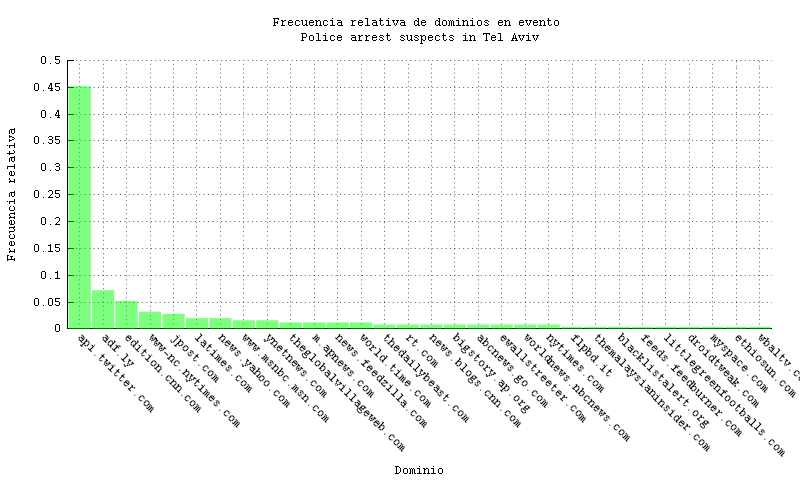
\includegraphics[width=14cm]{./img/telaviv-domain-freqs.png}
  \caption[Dominios evento 1]
   {Distribución de frecuencias de dominios del evento ``Police Arrest
  suspects in Tel Aviv"\label{fig:telaviv-domains}. Las frecuencias son relativas al total de
  documentos correspondientes al evento. Se puede apreciar rápidamente
  que la mayoría de los documentos tienen enlaces a Twitter.}
\end{figure}

\begin{itemize}
\item En la Figura \ref{fig:telaviv-domains} se aprecia una gran
      mayoría de documentos que tienen como URL \texttt{api.twitter.com}, lo
      cual significa que los tweets de esos documentos no presentaron
      ninguna URL en su contenido (dado que esos tweets pasan a
      representar un documento cuyo identificador es una URL que
      identifica al tweet que lo compone).

      En segundo lugar, la URL \texttt{adf.ly} tiene una segunda
      mayoría. \hyperref[sec-4.4.1]{Adf.ly} es un servicio de acortamiento de enlaces, con
      la característica de que el sitio muestra publicidad antes de
      mostrar el enlace a la URL a la cual apunta. Como no es una
      redirección directa, al tratar de resolver este dominio no fue
      posible recuperar destino final. Es posible suponer que los
      destinos de estas direcciones apuntan a más sitios de noticias,
      dadas los dominios que siguen a continuación, como CNN o NY
      Times.
\item De la misma forma, tanto para los eventos ``Clinton'' y
      ``Stockholm'', en las Figuras \ref{fig:clinton-domains} y
      \ref{fig:stockholm-domains}, la distribución de dominios sigue una tónica
      similar: la gran mayoría de documentos corresponden a un tweet
      de sólo texto, sin URL. Es posible que gran parte de los tweets
      hayan correspondido a texto debido a los términos de búsqueda
      que fueron utilizados para recuperarlos, tales como \texttt{clinton},
      \texttt{ceasefire}, \texttt{effort}, o \texttt{stockholm}.
\item Un caso especial ocurre para el evento ``New York'' en la Figura
      \ref{fig:dvorak-domains}. No hay una mayoría de documentos
      apuntando a Twitter: de hecho, la gran mayoría de los documentos
      posee una URL distinta, dada la proporción a la que se
      encuentran los dominios más frecuentes.
\end{itemize}
\begin{figure}[h]
  \centering
  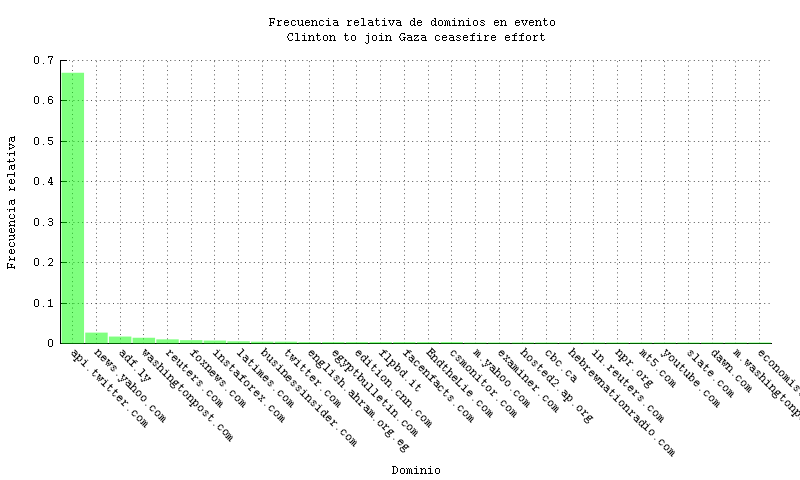
\includegraphics[width=14cm]{./img/clinton-domain-freqs.png}
  \caption[Dominios evento 2]
   {Distribución de frecuencias de dominios del evento ``Clinton to
  join Gaza ceasefire effort"\label{fig:clinton-domains}. Las frecuencias son relativas al total de
  documentos correspondientes al evento. Se puede apreciar rápidamente
  que la mayoría de los documentos tienen enlaces a Twitter.}
\end{figure}

\begin{figure}[h]
  \centering
  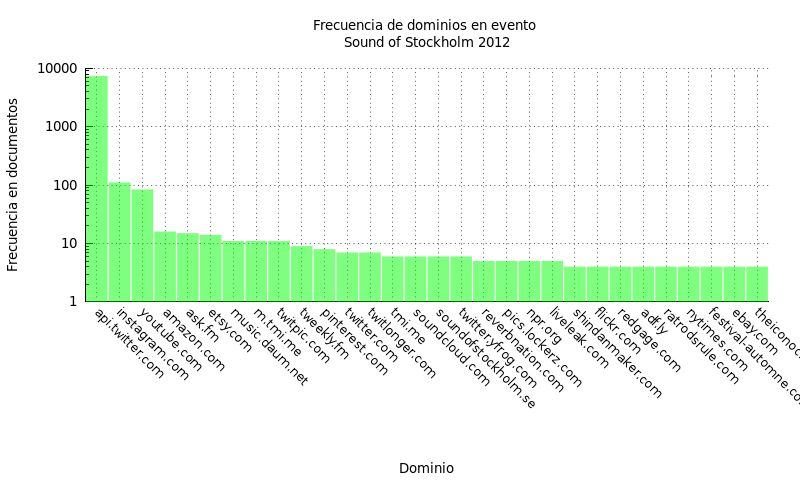
\includegraphics[width=14cm]{./img/stockholm-domain-freqs.png}
  \caption[Dominios evento 3]
   {Distribución de frecuencias de dominios del evento ``Sound of
  Stockholm 2012"\label{fig:stockholm-domains}. Las frecuencias son relativas al total de
  documentos correspondientes al evento. En este caso se quitó del
  gráfico lo que corresponde a Twitter, dejando los datos
  restantes. Se puede apreciar que los siguientes dominios representan
  no más del 10\% del total.}
\end{figure}

\begin{figure}[h]
  \centering
  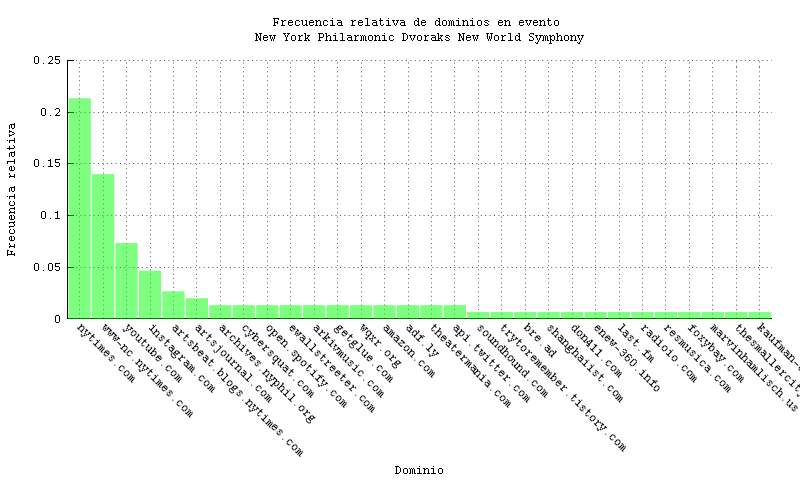
\includegraphics[width=14cm]{./img/dvorak-domain-freqs.png}
  \caption[Dominios evento 4]
   {Distribución de frecuencias de dominios del evento ``New York
  Philarmonic Dvorak's New World Symphony"\label{fig:dvorak-domains}. Las frecuencias son relativas al total de
  documentos correspondientes al evento.}
\end{figure}

\subsection{Determinar el número de clusters}
\label{sec-4.4.2}


Para determinar un número adecuado de clusters para cada evento se
utilizaron métricas de evaluación internas, dado que no se contó con
las clases reales de los datos obtenidos. Para esto, se utilizó el
software Cluto\footnote{\href{http://glaros.dtc.umn.edu/gkhome/views/cluto}{http://glaros.dtc.umn.edu/gkhome/views/cluto} }, el
cual ofrece varios algoritmos de clustering con medidas de evaluación
tanto internas (similitud intra-cluster y inter-cluster) como externas
(pureza y entropía).

La metodología utilizada para determinar el número de clusters fue la
siguiente:

\begin{itemize}
\item Calcular una solución de clustering particional usando
  $k \in \{2,\ldots,30\}$ clusters como parámetro.
\item Para cada solución obtenida, documentar la similitud intra-cluster
  promedio y inter-cluster promedio.
\item Determinar experimentalmente la solución con mayor similitud
  intra-cluster y menor similitud inter-cluster, calculando el radio
  entre estas dos medidas.
\end{itemize}
\begin{figure}[h]
  \centering
  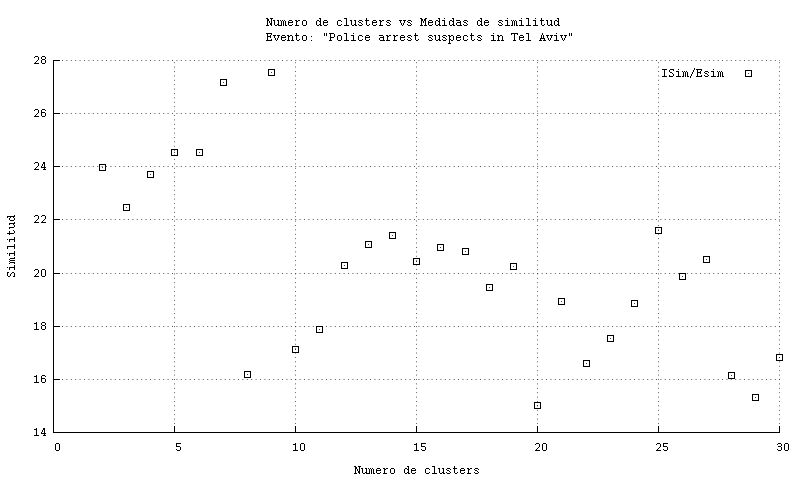
\includegraphics[width=14cm]{./img/telaviv-clusters-radio.png}
  \caption[Radios de similitud para evento 1]
   { Radio ISim/ESim del evento ``Tel Aviv". \label{fig:telaviv-radio}. }
\end{figure}

\begin{figure}[h]
  \centering
  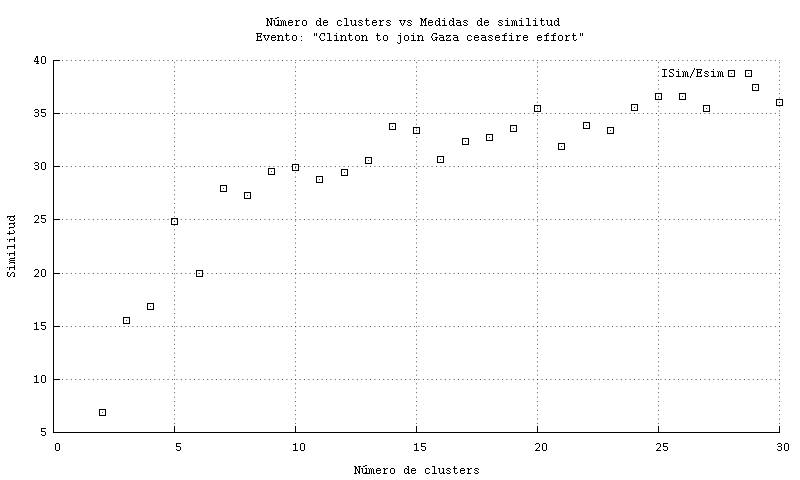
\includegraphics[width=14cm]{./img/clinton-clusters-radio.png}
  \caption[Radios de similitud para evento 2]
   { Radio ISim/ESim del evento ``Clinton". \label{fig:clinton-radio}. }
\end{figure}

\begin{figure}[h]
  \centering
  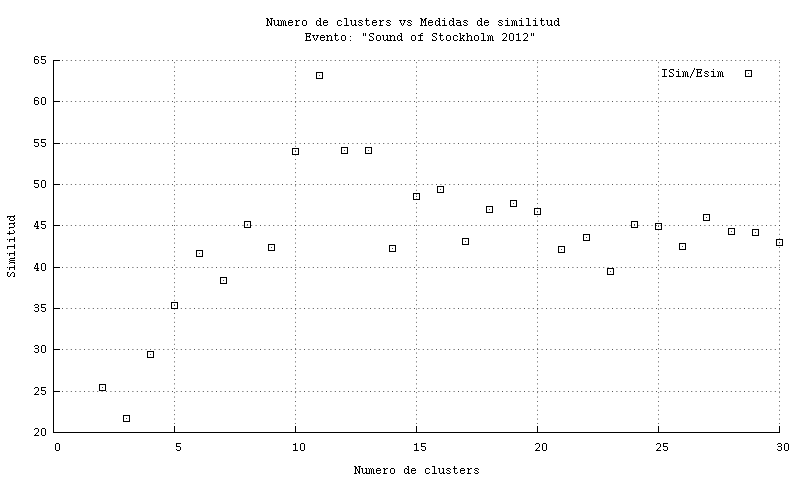
\includegraphics[width=14cm]{./img/stockholm-clusters-radio.png}
  \caption[Radios de similitud para evento 3]
   { Radio ISim/ESim del evento ``Stockholm". \label{fig:stockholm-radio}. }
\end{figure}

\begin{figure}[h]
  \centering
  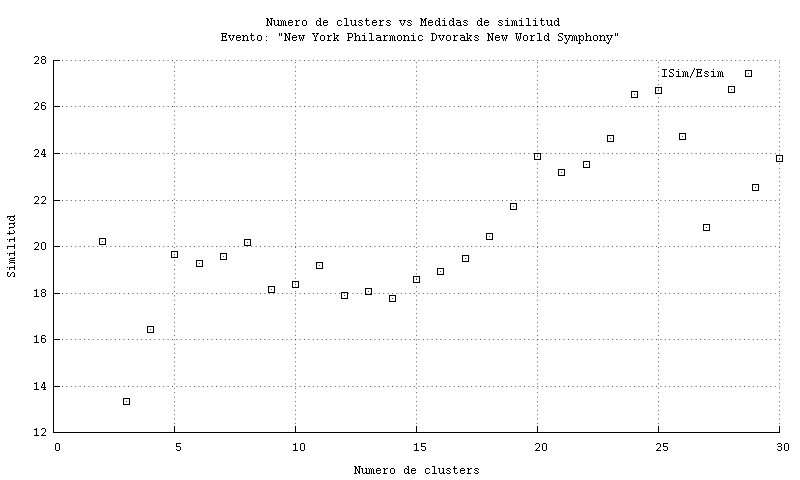
\includegraphics[width=14cm]{./img/dvorak-clusters-radio.png}
  \caption[Radios de similitud para evento 4]
   { Radio ISim/ESim del evento ``New York". \label{fig:dvorak-radio}. }
\end{figure}

Con esto, se puede determinar experimentalmente un número de clusters
para cada evento, y analizar los resultados obtenidos.

\subsection{Análisis de resúmenes}
\label{sec-4.4.3}


    Para analizar los resultados obtenidos, se generaron nuevamente
    clusterings utilizando el número estimado en la sección anterior, de
    forma de determinar una solución de mejor calidad.

    Una vez generados los clusterings, se procedió a hacer un análisis
    caso a caso de los resultados obtenidos.

    Por ejemplo, para el evento ``Tel Aviv'', se determinó como $9$ el
    número óptimo de clusters, dando como resultado una solución de
    clustering que particionaba los tweets de tal forma que cada
    cluster contenía principalmente sólo tweets del mismo tipo:

\begin{enumerate}
\item \texttt{Previous bomb attacks in Tel Aviv...}
\item \texttt{RT @BreakingNews: Israel's army spokesman says Israeli Arab        arrested for Wednesday's bus bombing in Tel Aviv}
\item Contiene tweets de distintos temas, tanto de Tel Aviv como
       otros relacionados a Israel, Egipto o Estados Unidos.
\item \texttt{RT @chaimlevinson: \#breakingnews : after massive  police hunt,        2  suspects in the tel aviv bus bombing arrested in 443 road}
\item \texttt{Police Arrest Suspects in Tel Aviv Bus Blast, Including        Israeli Citizen:}
\item \texttt{Israel arrests suspects in Tel Aviv bus bombing: Israeli}
       \texttt{authorities arrested an Israeli Arab on suspicion of planting a}
       \texttt{bomb in a Te...}
\item \texttt{Arrest announced in Tel Aviv bus bombing: An arrest has been}
       \texttt{made in Wednesday\textbackslash{}xe2\textbackslash{}x80\textbackslash{}x99s bombing in Tel Aviv of a bus,=        =a...}
\item \texttt{RT @panosharitos: Tel Aviv police chasing after two suspects}
       \texttt{(one arrested), say this was not a suicide bombing; 3 of the}
       \texttt{casualties are ...}
\item \texttt{Shin Bet, police arrest suspects in Tel Aviv bus bombing}
       \texttt{http://t.co/hJzLAOnD}
\end{enumerate}
    Los mensajes expuestos son los más frecuentes dentro de su
    cluster, a excepción del cluster n°2, que contenía tweets con
    distintos temas.

    Los resultados del ranking sobre cada cluster entrega
    efectivamente los tweets más ``populares'' dentro de los indicadores
    escogidos (número de retweets, autoridad de la cuenta, etc.). En
    la Figura \ref{fig:bn} se puede apreciar el documento con más
    puntaje obtenido por el ranking. Su alto puntaje se debió
    principalmente a la cantidad de retweets y a que el autor es una
    cuenta verificada.

\begin{figure}[h!]
  \centering
  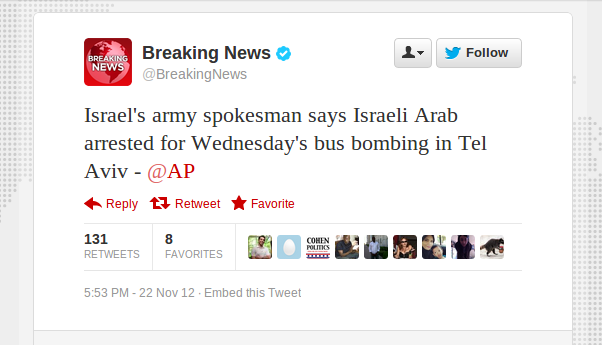
\includegraphics[width=10cm]{./img/breakingnews.png}
  \caption[Documento con alto puntaje entre los resultados obtenidos]
   { Documento (tweet) con más relevancia dentro del evento ``Tel Aviv". \label{fig:bn} }
\end{figure}

    Siguiendo con los resultados, para el evento ``New York'', el cual consiste en un
    concierto musical de la Filarmónica de Nueva York, a pesar de la
    poca cantidad de documentos (250), los resultados también fueron
    muy representativos e incluso ricos en contenido multimedia. En la
    Figura\footnote{Fuente \href{http://instagram.com/p/SF8w-3voOF/}{http://instagram.com/p/SF8w-3voOF/} }
    \ref{fig:dvorak} se puede apreciar uno de los resultados; además
    de este se incluyen artículos de prensa, vídeos de YouTube,
    grabaciones en servicios de sonido o música como Soundcloud,
    Spotify o Shazam.

    Por otra parte, sin embargo, al analizar los resultados del evento
    ``Stockholm'', que tiene cerca de ocho mil documentos, se notó que
    gran parte de ellos corresponden a tweets sin sentido con el tema,
    o bien tweets de contenido personal que no tenían ninguna
    relación. Estos tweets alcanzaron alta relevancia debido a altos
    indicadores: autoridad de usuarios, cantidad de followers y en
    ocasiones cantidad de retweets. Esto indica que la forma de
    realizar ranking puede ser mejorada en otros aspectos, quizás
    considerando el contenido del tweet directamente o de alguna
    manera verificando la relevancia del documento mencionado.

\begin{figure}[h!]
  \centering
  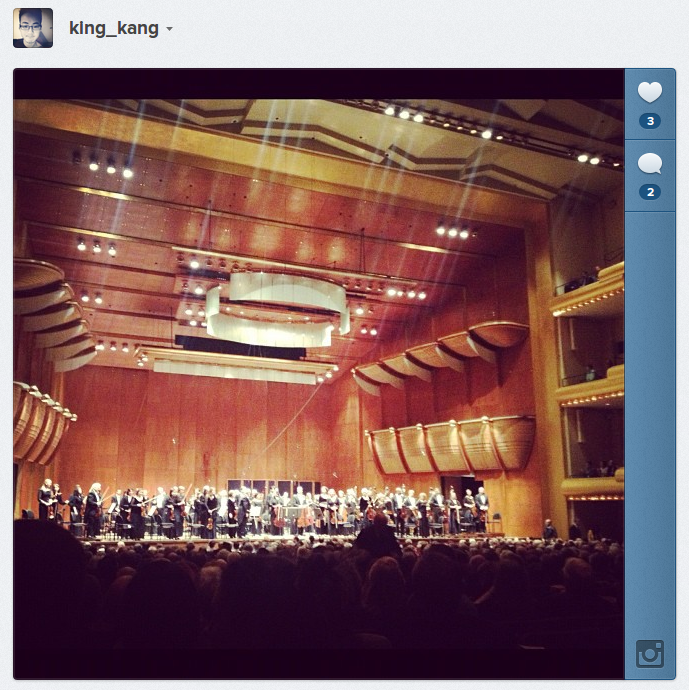
\includegraphics[width=8cm]{./img/dvorak.png}
  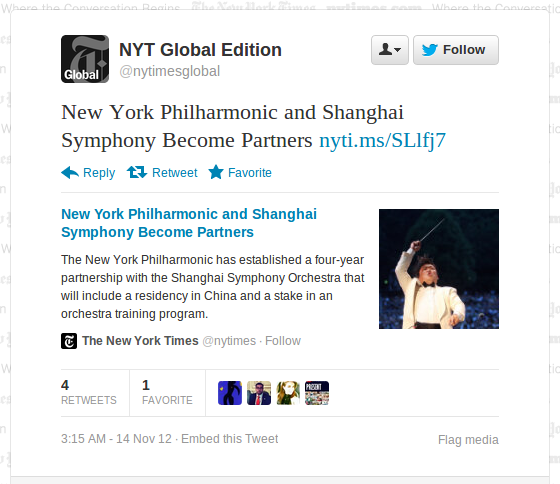
\includegraphics[width=8cm]{./img/dvorak2.png}
  \caption[Imagen y documento con altos puntajes entre los resultados obtenidos]
   { Documento (fotografía) y tweet con alta relevancia dentro del evento
  ``New York". \label{fig:dvorak} }
\end{figure}

    Finalmente, el evento ``Clinton'' obtuvo buenos resultados, en su
    mayoría tweets sin URL, que discuten nuevamente el tema de
    Gaza. Sin embargo, los medios de prensa mencionados en las URLs
    consideran contenido multimedia (imágenes y vídeos), sin embargo,
    se consideró esto anecdótico. La característica de este evento es
    su alto contenido textual en la forma de consignas respecto al
    tópico que discuten.
\chapter{Conclusiones}
\label{sec-5}

\section{Resumen del trabajo realizado}
\label{sec-5.1}

\section{Objetivos alcanzados}
\label{sec-5.2}

\section{Relevancia del trabajo realizado}
\label{sec-5.3}

\section{Trabajo futuro}
\label{sec-5.4}


\begin{comment}
\chapter{Conclusión}
\lipsum[130-132]
\begin{figure}[!h]
\centering

\includegraphics[scale=.2]{fcfm}
\caption{Logo de la Facultad}
\label{logofcfm}
\end{figure}
\lipsum[133-134]
\begin{table}[!h]
\centering
\begin{tabular}{|c||c|}
\hline
Campo 1& Campo 2\\\hline
Valor 1& Valor2\\\hline
\end{tabular}
\caption{Tabla 1}
\label{tabla:1}
\end{table}
\lipsum[135]
\end{comment}

\nocite{*}
\bibliographystyle{plain}
\bibliography{bibliografia}

%\chapter{Anexos}
\end{document}
